\title{Year 12 Chemistry Depth Study}
\author{
NESA \#: 34364338 
}

\documentclass[12pt, a4paper]{article}
\usepackage[margin=0.5in]{geometry}
\usepackage{parskip}
\usepackage{amsmath}
\usepackage[T1]{fontenc}

\usepackage{graphicx}
\graphicspath{ {./images/} }

\begin{document}
\maketitle

\begin{abstract}
This depth study report explores the role of equilibrium systems and reversible reactions within industrial applications, including the Contact Process and the Solvay Process.
\end{abstract}




\section{Contact Process}

The Contact Process is a multi-step industrial process used to produce concentrated sulfuric acid. 

\begin{enumerate}
	\item Produce sulfur dioxide from sulfur and excess oxygen
	\item Convert sulfur dioxide to sulfur trioxide
	\item Produce oleum (fuming sulfuric acid) from sulfur trioxide
	\item React oleum with water to produce concentrated sulfuric acid
\end{enumerate}

\subsection{Exploring the Contact Process}

\subsubsection{Producing sulfur dioxide}

To produce sulfur dioxide, an irreversible exothermic combustion reaction between sulfur and oxygen is used to produce sulfur dioxide.

\begin{align}
	S(s) + O_{2}(g) \rightarrow SO_{2}(g)
\end{align}

\subsubsection{Sulfur dioxide to sulfur trioxide}

The conversion of sulfur dioxide to sulfur trioxide is an exothermic reversible reaction, generally performed in a contact tower or oxidation chamber.

\begin{align}
	2SO_{2}(g) + O_{2} \rightleftharpoons 2SO_{3}(g) \qquad \qquad \Delta H = -196 \; kJ \; mol^{-1}
\end{align}

A catalyst of \textbf{vanadium(V) oxide} is used to reduce the activation energy, hence reducing the energy used for the reaction.

\pagebreak

\subsubsection{Producing concentrated sulfuric acid}

After the production of sulfur trioxide, sulfuric acid is produced in an absorption tower. For a more stable reaction, sulfur trioxide is first dissolved in concentrated sulfuric acid, to produce \textbf{oleum} (or fuming sulfuric acid). Without this initial step, the reaction would produce sulfuric acid gas (as a mist or vapor) as the reaction would be highly exothermic.

\begin{align}
	H_{2}SO_{4}(l) + SO_{3}(g) \rightarrow H_{2}S_{2}O_{7}(l)
\end{align}

Once oleum is produced, it is safely reacted with water to produce concentrated sulfuric acid, in a dilution tank.

\begin{align}
	H_{2}S_{2}O_{7}(l) + H_{2}O(l) \rightarrow 2H_{2}SO_{4}(l)
\end{align}

As indicated by the molar ratio in reactions (3) and (4), the production of concentrated sulfuric acid from oleum produces twice as much concentrated sulfuric acid, as what was originally used to produce oleum.

\subsection{The importance and uses of sulfuric acid}

Sulfuric acid is a key primary product used to produce a number of other chemical compounds, and the Contact Process allows them to be produced efficently in high concentrations at industrial scales. 

\paragraph{Fertilisers}
Sulfuric acid is a key reactant for the production of phosphate-based fertilisers. For example, calcium phosphates are often used as fertiliser and is produced by reacting phosphorite with sulfuric acid.

\begin{align}
	Ca_{3}(PO_{4})_{2}(s) + H_{2}SO_{4}(aq) \rightarrow Ca(H_{2}PO_{4})_{2}(s) + 2CaSO_{4}(s)
\end{align}

Phosphate-based fertilisers are critical to the world's food supply, in ensuring that there is enough food production to sustain a growing world population. According to researchers, without phosphate and nitrogen-based fertilisers, humanity would only be able to produce half its current food production.\footnote{Faradji \& de Boer, 2016.}

\paragraph{Cleaning agents}
Outside of fertiliser, sulfuric acid is also used as an industrial cleaning agent. It helps to remove oxidation and rust from iron and steel-based components in the passenger motor vehicles (PMV) and major appliances industries, while also featuring as an ingredient in some household cleaning agents such as drain cleaners.

\subsection{Factors affecting equilibrium}

\textbf{Le Chatelier's Principle} states that within equilibrium, a disturbance caused by changing conditions (such as temperature, pressure and concentration) will result in an \textbf{equilibrium shift} to counteract and re-establish the equilibrium. In the case of the Contact Process, it features one \textbf{equilibrium reaction}: the conversion of sulfur dioxide to sulfur trioxide.

\begin{align}
	2SO_{2}(g) + O_{2} \rightleftharpoons 2SO_{3}(g) \qquad \qquad \Delta H = -196 \; kJ \; mol^{-1}
\end{align}

\subsubsection{Temperature}

The forward reaction is \textbf{exothermic} (\(\Delta H = -196 \; kJ \: mol^{-1}\)). By \textbf{Le Chatelier's Principle}, lowering temperature will favour the exothermic side of the reaction. Hence, as temperature decreases, the equilibrium shifts right and the disturbance of the equilibrium is counteracted by an increase in the production of sulfur trioxide. 

However, as temperature decreases, there is less kinetic energy and less frequent successful collisions, hence the rate of reaction decreases (as increased energy is required to break bonds). Therefore, to produce a reasonably high yield at a fast rate, a higher compromise temperature of 400°C to 450°C is often used in industrial applications. As seen in the provided graph, this temperature will gain 80-90\% yield, with minimal yield increases as temperature approaches zero.

\begin{center}
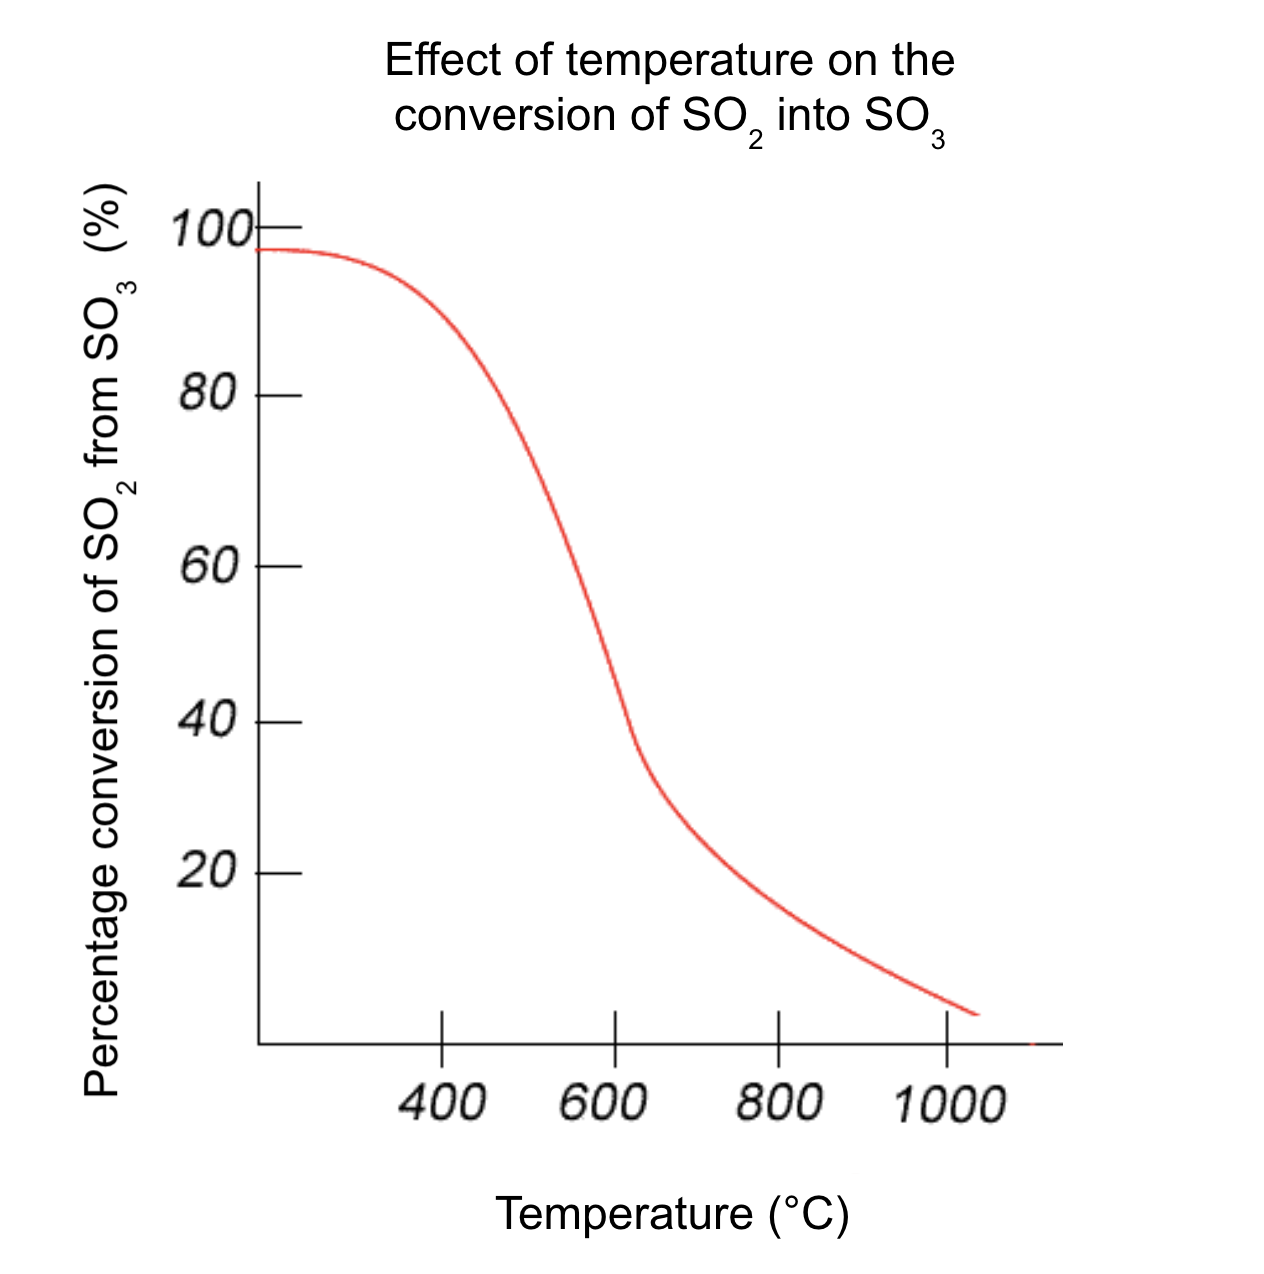
\includegraphics[scale=0.5]{graph}
\end{center}

\subsubsection{Pressure}

By \textbf{Le Chatelier's Principle}, an increase in pressure will favour the side with fewer number of moles. In this case, this is the products side, and the equilibrium shifts right. The system will then counteract the disturbance by decreasing pressure, both increasing the rate of reaction, as well as producing more sulfur trioxide.

However, low pressure can still garner an extremely high rate of sulfur dioxide to sulfur trioxide. In industrial applications, lower pressures are used, as they still generate high yield (99.5\%) and often it is economically not justifiable to invest in substantially higher pressures for minimal yield gain.

\subsubsection{Concentration}

By \textbf{Le Chatelier's Principle}, an increase in concentration in one side will lead to a shift to the opposite side. Using a 1:1 proportion of sulfur dioxide to oxygen would place oxygen in excess and cause a shift to the right. Therefore, increasing the concentration of oxygen gas (a reactant) will produce more sulfuric trioxide. 

\subsubsection{Catalyst}

\textbf{Catalysts} lower the activation energy required for the reaction to take place, increasing the rate of reaction. By lowering the activation energy, the bonds in the reactants weaken, thereby increasing the rate of reaction, and eliminating the need for otherwise-needed expensive high-pressure systems.

Within the equilibrium reaction, a catalyst of vanadium(V) oxide (\(V_{2}O_{5}\)) is used for a reversible reaction, enabling a dynamic equilibrium to be established. Without a catalyst, the reaction would virtually remain at a static equilibrium.

\section{Solvay Process}

The Solvay Process is a synthsis reaction which reacts carbon dioxide (produced from limestone), ammonia and brine to produce sodium carbonate.



\pagebreak

\section{Bibliography}

British Broadcasting Corporation 2021, Sulfuric acid and the contact process, viewed 17 October 2021, \\ \textless{https://www.bbc.co.uk/bitesize/guides/zb7f3k7/revision/1}\textgreater

Clark, Jim 2021, \emph{The Contact Process}, Truro School in Cornwall, viewed 17 October 2021, \\ \textless{https://chem.libretexts.org/@go/page/3838}\textgreater

Department of Agriculture, Water and the Environment 2019, Sulfuric acid, Commonwealth of Australia, viewed 18 October 2021, \textless{http://www.npi.gov.au/resource/sulfuric-acid}\textgreater

Faradji, Charly \& de Boer, Marissa 2016, \emph{How the great phosphorus shortage could leave us all hungry}, The Conversation, viewed 18 October 2021, \\ \textless{https://theconversation.com/how-the-great-phosphorus-shortage-could-leave-us-all-hungry-54432}\textgreater

IB Chemistry Web, Equilibrium: Industrial Processes 2016, viewed 22 October 2021, \\ \textless{https://www.ibchem.com/IB16/07.27.htm}\textgreater

Manahan, S E 2016, \emph{Industrial Chemical Reactions - The Solvay Process}, University of Missouri, viewed 24 October 2021 \\ \textless{https://chem.libretexts.org/@go/page/285417}\textgreater

Royal Society of Chemistry n.d., 

The Essential Chemistry Industry 2016, Sulfuric acid, viewed 18 October 2021, \\ \textless{https://www.essentialchemicalindustry.org/chemicals/sulfuric-acid.html}\textgreater

Vedantu, Contact Process n.d., viewed 22 October 2021, \\ \textless{https://www.vedantu.com/iit-jee/contact-process}\textgreater

Wansbrough, H \& Simpson, J \& Petherick, J \& Donaldson, L 2017, \emph{The Manufacture of Sulfuric Acid and Superphosphate}, New Zealand Institute of Chemistry, viewed 24 October 2021, \\ \textless{https://nzic.org.nz/app/uploads/2017/10/1B.pdf}\textgreater

Wikipedia contributors 2021, \emph{Contact process}, Wikipedia, the Free Encyclopedia, viewed 22 October 2021, \\ \textless{https://en.wikipedia.org/w/index.php?title=Contact\_process\&oldid=1047723670}\textgreater

\end{document}

==================================================

inline notes:

- are we doing solvay process?
- manually use bibliography because the high school is too basic for bibtex :( - no Harvard AU support + they don't like [n]
- format date{today} later 
- check contact process concentration
- cut down word count
